\section{Рабочий проект}
\subsection{Классы, используемые для разработки редактора}

Можно выделить следующий список классов и их методов, использованных при разработке web-приложения (таблица \ref{class:table}). Пример таблицы с уменьшенным межстрочным интервалом.

\renewcommand{\arraystretch}{0.9} % уменьшение расстояний до сетки таблицы
\begin{xltabular}{\textwidth}{|X|p{2.5cm}|>{\setlength{\baselineskip}{0.7\baselineskip}}p{4.85cm}|>{\setlength{\baselineskip}{0.7\baselineskip}}p{4.85cm}|}
	\caption{Описание классов, используемых в приложении\label{class:table}}\\
	\hline \centrow \setlength{\baselineskip}{0.7\baselineskip} Название класса & \centrow \setlength{\baselineskip}{0.7\baselineskip} Модуль, к которому относится класс & \centrow Описание класса & \centrow Методы \\
	\hline \centrow 1 & \centrow 2 & \centrow 3 & \centrow 4\\ \hline
	\endfirsthead
	\caption*{Продолжение таблицы \ref{class:table}}\\
	\hline \centrow 1 & \centrow 2 & \centrow 3 & \centrow 4\\ \hline
	\finishhead
	Application & app.py &  Этот класс представляет главное приложение ALGOLIB & \_init\_(root: CTk), open\_admin(),ask\_pass(), check\_pass(entered\_pw),	update\_password(), user\_interface(), return\_to\_main\_page() ,update\_algorithm\_list(), admin\_interface(), change\_password() ,confirm\_pw\_change(), add\_algorithm(), confirm\_add\_algorithm()
	,modify\_algorithm(), update\_content(), submit\_content(), delete\_algorithm().

	\hline  MyFrame & my\_frame.py & Этот класс представляет рамку, содержащую алгоритмы.  & \_init\_(master,textbox, **kwargs),	create\_buttons(), update\_filtered\_alg(), show algorithm(), master: Tktoplevel, textbox: Gtktextbox, all\_algorithms: list, filtered\_algorithms:, listen
	
	
	
	\hline CTk Messagebox & CTkMes- sageboxь & Этот класс представляет окно сообщения. Он отображает сообщения для пользователя. & Имеет дополнительные две точки для cross и init.
	
 \end{xltabular}
\renewcommand{\arraystretch}{1.0} % восстановление сетки



\subsection{Системное тестирование алгоритмической библиотеки .}
\begin{enumerate}
	
	\item Случай использования «алгоритм поиска»:
	\begin{itemize}
		\item основной исполнитель: пользователь;
		\item заинтересованные лица и их требования: пользователю необходимо добавить определенную фигуры на окно редактора;
		\item предусловие: пользователь открыл растровый редактор;
		\item ожидаемый результат: пользователь нажимает нужную горячую клавишу, ставит две координатные точки фигуры с помощью мышки, после этого фигура появляется на окно редактора. В итоге на окно редактора добавлятся выбранный пользователем геомерический обьект.
		\item результат представлен на рисунке 4.1
	\end{itemize}
	
	

	\begin{figure}[H]
		\centering
		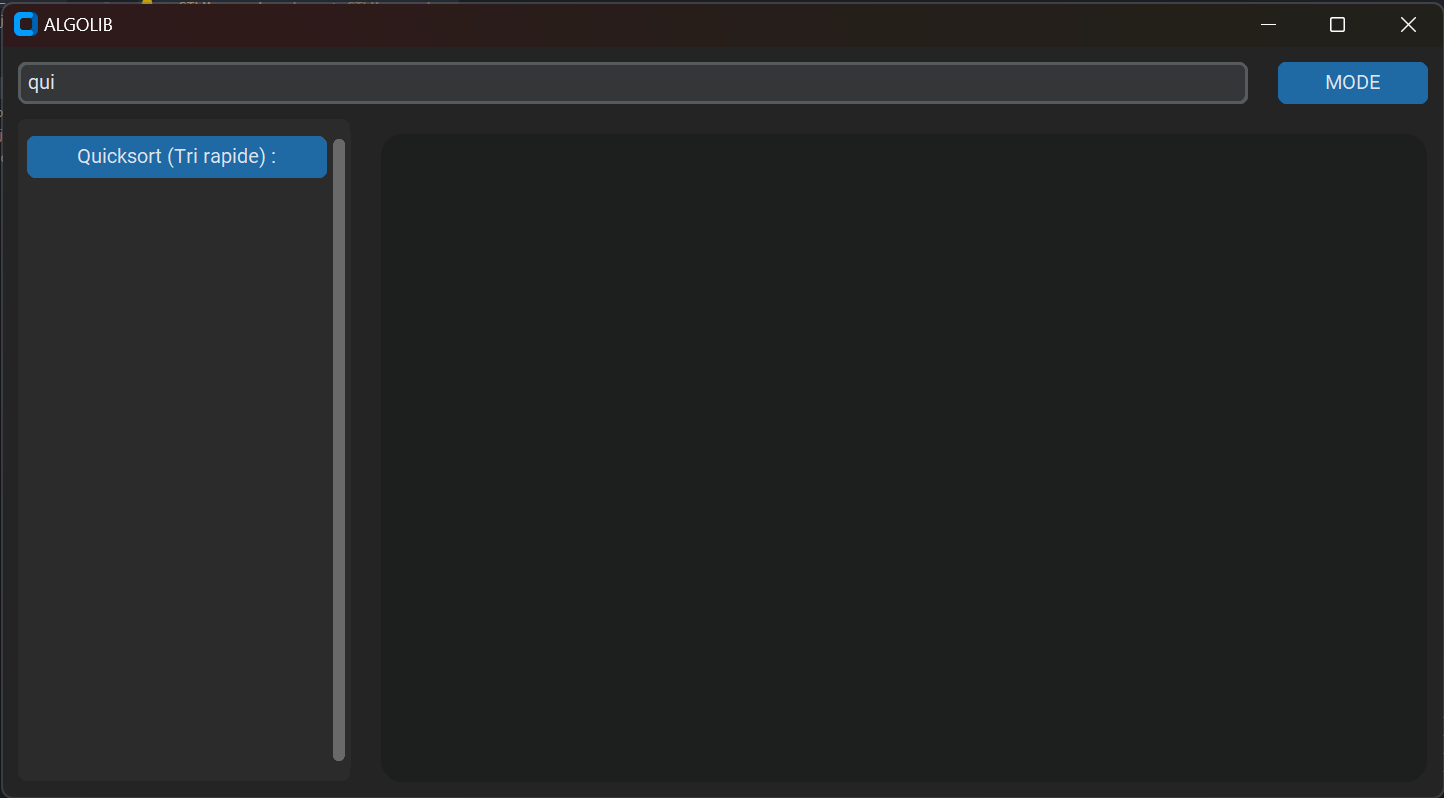
\includegraphics[width=0.7\linewidth]{images/adding}
		\caption{алгоритм поиска}
		\label{fig:classdiag}
	\end{figure}
	
	\item Случай использования «Удаление геометрического обьекта»:
	\begin{itemize}
		\item вариант использования "показать содержимое алгоритма"
		\item главный исполнитель: пользователь;
		\item заинтересованные стороны и их требования: пользователь нажимает кнопку в алгоритме, который он хочет;
		\item предварительное условие: пользователь открыл алгоритмическую библиотеку.
		\item ожидаемый результат: отображается описание географии.
			\item результат показан на рисунке 4.2.
	\end{itemize}
	
	\begin{figure}[H]
		\centering
		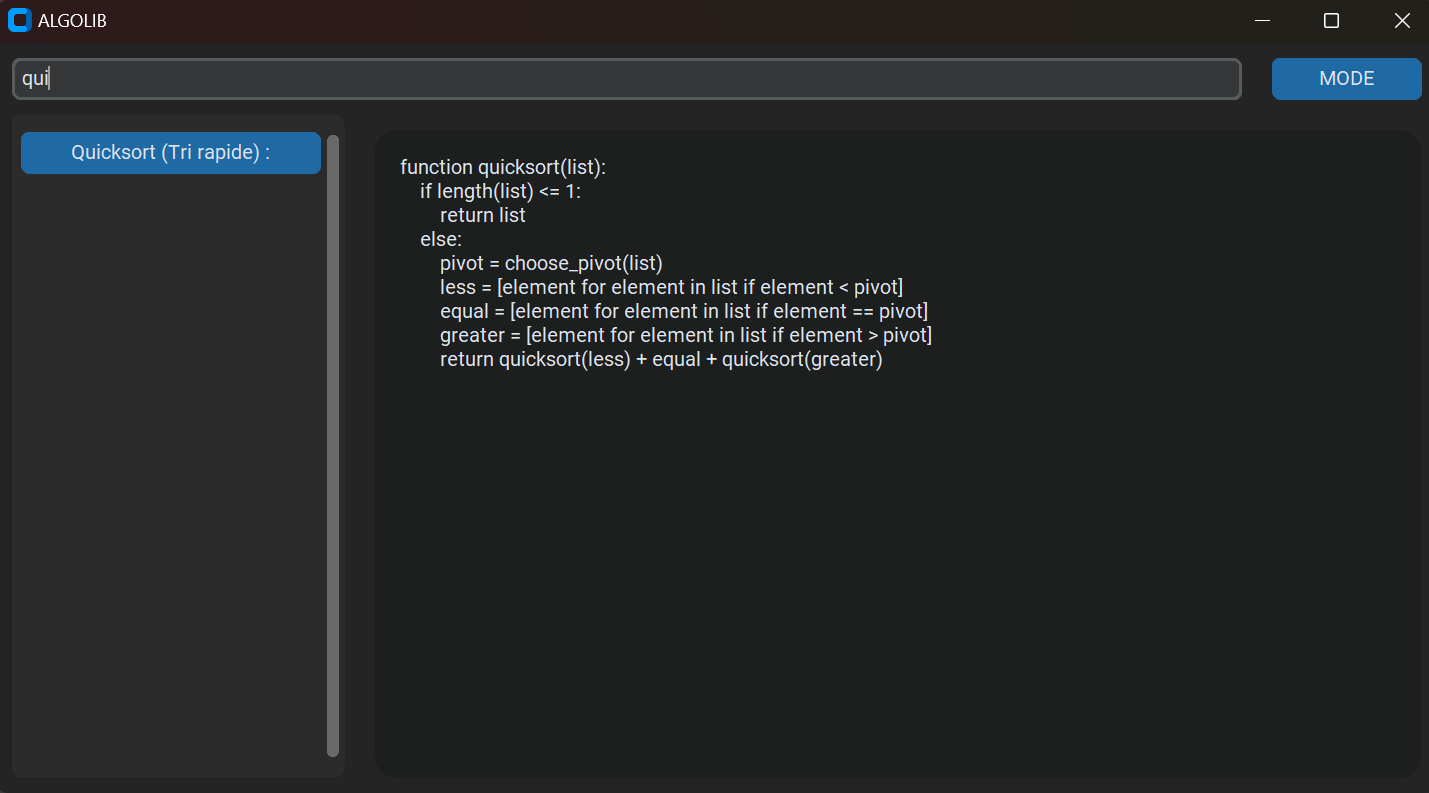
\includegraphics[width=0.7\linewidth]{images/delete}
		\caption{показан на рисунке }
		\label{fig:classdiag}
	\end{figure}
	
	
	
\end{enumerate}
